Wenn es unterschiedlich lang auf dem Sourcedatensatz trainiert wird, fällt auf, dass das Netz unterschiedlich gut auf dem Targetdatensatz ist. 
Da es sowieso ausgestestet werden muss, wann TF genutzt wird, wird nun das ConvMaxPool-Netzwerk genommen und nach jedem Layer TF angewandt. 
Das Ergebnis davon ist in Figure 3.5 zu sehen. 

\begin{figure}[htpb]
    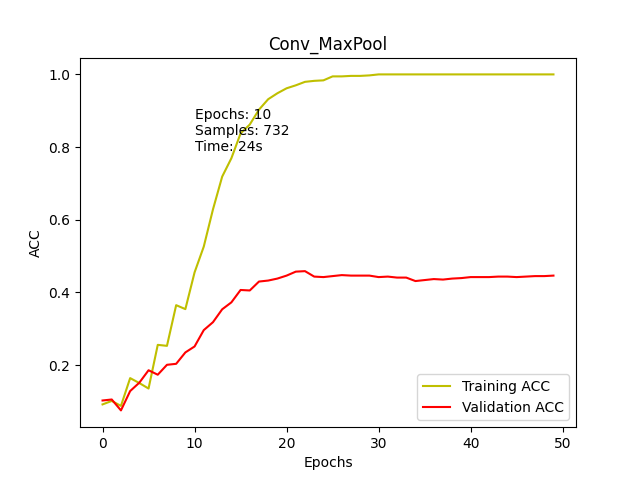
\includegraphics[height=5cm]{../../Plots/ba_plots/convmaxpool/wotr.png}
    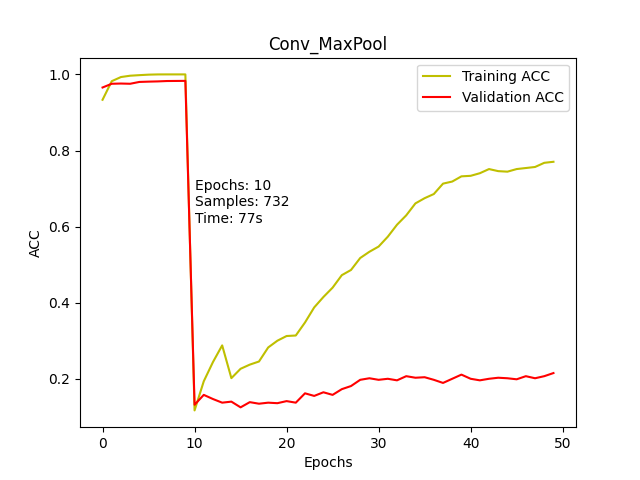
\includegraphics[height=5cm]{../../Plots/ba_plots/convmaxpool/1TFtr.png}
    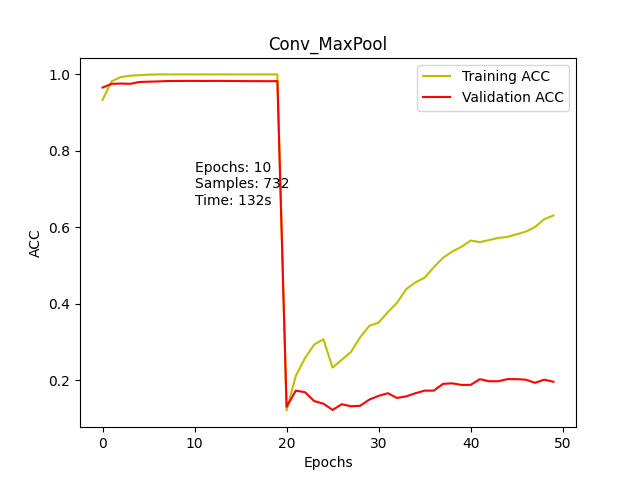
\includegraphics[height=5cm]{../../Plots/ba_plots/convmaxpool/2TFtr.png}
    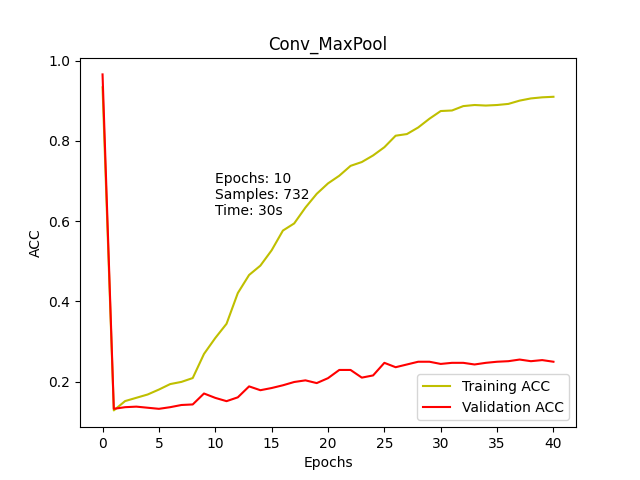
\includegraphics[height=5cm]{../../Plots/ba_plots/convmaxpool/epochTFtr.png}
    % 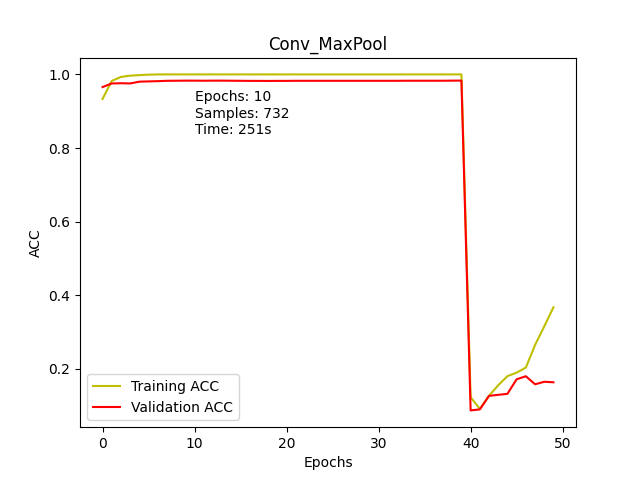
\includegraphics[height=5cm]{../../Plots/ba_plots/convmaxpool/4TFtr.png}
    \caption{\label{fig:layertf} TF bei unterschiedlichen Layern}
\end{figure}

Auffällig ist es, dass hier die beste Performanz ohne TF ist. Bereits nach nur einer Epoche im ersten Layer, welches auf dem Sourcedatensatz 
trainiert wird, bricht die Accuracy ein. Dies zeigt, dass TF bei Klassifikation und Deep Cascade Netzwerken sinnfrei ist. Das 
Trainingsset der Trainingsdaten ist bei TF nie auch nur annähernd an den Bereich kommt, in dem es bei ohne TF ist. Daraus folgt, dass es 
bereits zu Overfitting auf dem Sourcedatensatz gekommen ist. Dadurch kann nicht mehr so gut auf dem Targetdatensatz gelernt werden. Dieses 
Overfitting passiert sogar bereits, wenn nur eine Epoche auf dem Sourcedatensatz gelernt wird, was die letzte Graphik von Figure 3.4 zeigt. 
Ebenso ist es offensichtlich, dass es bei jedem Graph zu Overfitting auf dem Trainingsset des Targetdatensatzes kam, da dieser um 60\% höhere 
Accuracy als das Validationset und dem Testdatenset vorweist. 

Bei einem Regressionnetzwerk, wie dem Deep Cascade Netzwerk RegressionTwo kommt es, wie in Figure 3.6 zu sehen, nicht so schnell zu Overfitting. 
Weder auf dem Sourcedatensatz noch auf dem Targetdatensatz. 

\begin{figure}[htpb]
    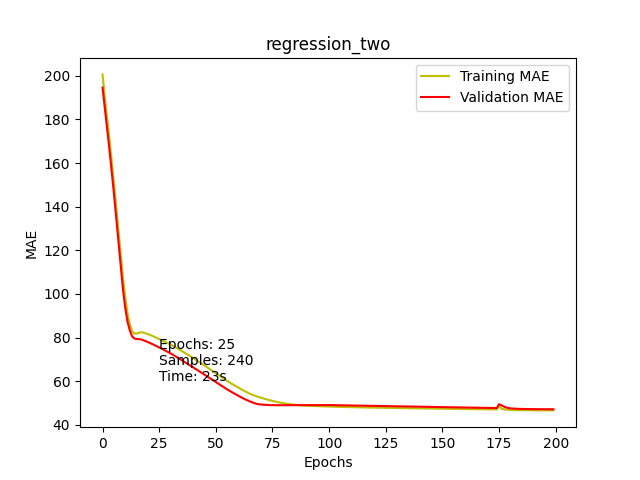
\includegraphics[height=5cm]{../../Plots/ba_plots/regr2/woregr2tr.png}
    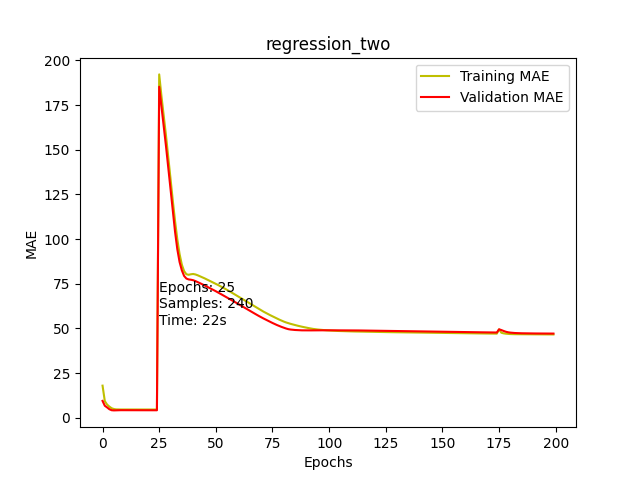
\includegraphics[height=5cm]{../../Plots/ba_plots/regr2/1TFtr.png}
    \caption{\label{fig:regr2tf} TF bei Regression}
\end{figure}

Dieses Overfitting-Problem hat nur die Klassifikation. Dies muss an der Loss-Function, die für Klassifikation benutz wird, liegen. Also 
am CategoricalCrossEntropy. Dahinter ist folgende Formel: 

\begin{equation}
    CCE = -\frac{1}{M}*\sum_{k=1}^{K}\sum_{m=1}^{M}*y_m^k * \log(h_w(x_m, k))
\end{equation} 

Dabei ist M die Anzahl der Datensamples, K die Anzahl der Klassen, $y_m^k$ das Target label, x der Input und $h_w$ die 
Gewichte \cite{rwcrossentropy}.

